\documentclass[11pt]{article}

% Packages
\usepackage[margin=1in, top=0.7in]{geometry}
\usepackage{amsmath,amssymb,amsfonts}
\usepackage{graphicx}
\graphicspath{{./}{../}}
\usepackage{hyperref}
\usepackage{algorithm}
\usepackage{algpseudocode}
\usepackage{booktabs}
\usepackage{longtable}
\usepackage{multirow}

% Document info
\title{Assignment 2 Report\\
    CS-726: Advanced Machine Learning}
\author{Deeptanshu Malu \quad Deevyanshu Malu \quad Neel Rambhia}
\date{}

\begin{document}

\maketitle

\section{Denoising Diffusion Probabilistic Models}

\subsection{Architecture}

The implemented Denoising Diffusion Probabilistic Model (DDPM) architecture consists of several key components:

\subsubsection{Time Embedding}
We use sinusoidal position embeddings to encode timestep information:
\begin{itemize}
    \item The \texttt{SinusoidalPositionEmbeddings} module transforms scalar timesteps into 16 dimensional embeddings
    \item This creates a unique representation for each timestep that preserves the notion of time progression
    \item The embedding uses a combination of sine and cosine functions at different frequencies, allowing the model to distinguish between timesteps
\end{itemize}

\subsubsection{Network Architecture}
The model consists of:
\begin{itemize}
    \item An input linear layer that maps the concatenation of data and time embeddings to a hidden dimension (128 units)
    \item A series of 5 \texttt{DiffusionBlocks}, each containing a linear layer of 128 units followed by a ReLU activation
    \item An output linear layer that maps back to the data dimensionality
\end{itemize}

Rather than using convolutional layers as in image-based diffusion models, we use fully connected layers which is appropriate for dataset without temporal or spatial structure. The time embedding ensures the model can adapt its behavior based on the specific noise level at each timestep.

\subsection{Results}

For NLL caluclation, the temperature is set to 0.1.
For EMD calculation, the number of subsamples is set to 250 and the number of iterations is set to 5.

For all training runs, the hyperparameters used are as follows:
\begin{itemize}
    \item \textbf{Epochs}: 100
    \item \textbf{Batch Size}: 64
    \item \textbf{Learning Rate}: 1e-3
    \item \textbf{Number of Samples}: 5000
\end{itemize}

\subsubsection{Varying Timesteps}
Here, lbeta = 0.0001 and ubeta = 0.02.

\begin{longtable}{|l|l|c|c|c|c|c|c|}
    \hline
    \textbf{Dataset} & \textbf{Metric} & \multicolumn{6}{c|}{\textbf{Timesteps}} \\
    \cline{3-8}
    & & \textbf{10} & \textbf{50} & \textbf{100} & \textbf{150} & \textbf{200} & \textbf{500} \\
    \hline
    \multirow{2}{*}{Moons} & EMD & 39.99 & 28.95 & \textbf{27.40} & 29.64 & 30.55 & 44.90 \\
    \cline{2-8}
    & NLL & 1.02 & 0.96 & 0.94 & \textbf{0.93} & 0.94 & 0.95 \\
    \hline
    \multirow{2}{*}{Circles} & EMD & 34.60 & \textbf{31.48} & 33.24 & 34.41 & 38.62 & 42.04 \\
    \cline{2-8}
    & NLL & 1.05 & 0.99 & 1.00 & \textbf{0.98} & 1.01 & 1.03 \\
    \hline
    \multirow{2}{*}{Blobs} & EMD & 88.78 & 43.69 & 20.08 & 18.36 & \textbf{17.17} & 19.83 \\
    \cline{2-8}
    & NLL & 0.34 & 0.12 & 0.04 & 0.03 & \textbf{0.01} & 0.04 \\
    \hline
    \multirow{2}{*}{Manycircles} & EMD & 33.65 & \textbf{26.41} & 27.77 & 27.98 & 30.98 & 30.34 \\
    \cline{2-8}
    & NLL & 0.66 & \textbf{0.54} & \textbf{0.54} & \textbf{0.54} & \textbf{0.54} & 0.58 \\
    \hline
    \multirow{2}{*}{Helix} & EMD & 56.00 & 59.33 & 57.15 & \textbf{56.13} & 58.87 & 60.49 \\
    \cline{2-8}
    & NLL & 1.55 & 1.53 & 1.52 & 1.52 & 1.53 & \textbf{1.51} \\
    \hline
    \caption{EMD and NLL values for DDPM with varying timesteps.}
\end{longtable}

For most datasets, there's a sharp improvement in both EMD and NLL when moving from T=10 to T=50 or T=100. This suggests that too few timesteps lead to poor approximation of the reverse diffusion process. But after reaching an optimal point, further increases in timesteps provide marginal or even negative returns.


\begin{figure}[H]
    \centering
    \begin{tabular}{ccc}
        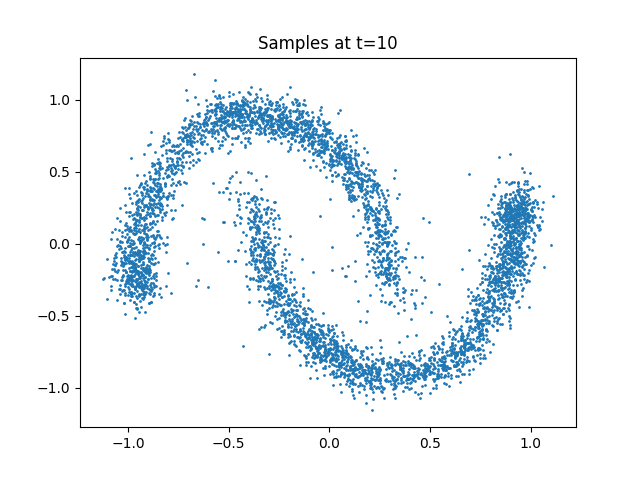
\includegraphics[width=0.3\textwidth]{exps/ddpm_2_10_0.0001_0.02_moons/samples_10.png} &
        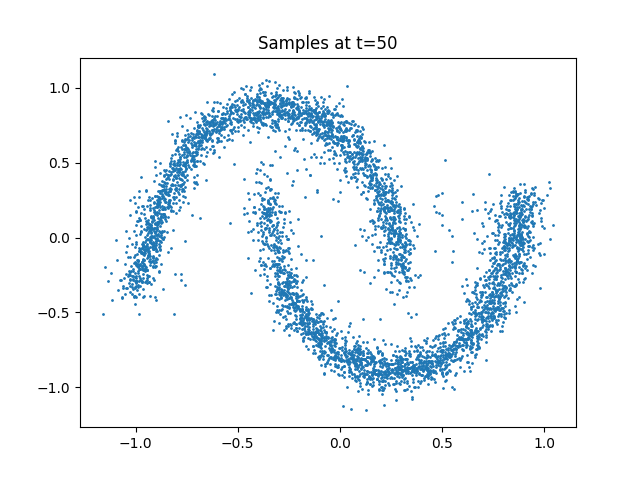
\includegraphics[width=0.3\textwidth]{exps/ddpm_2_50_0.0001_0.02_moons/samples_50.png} &
        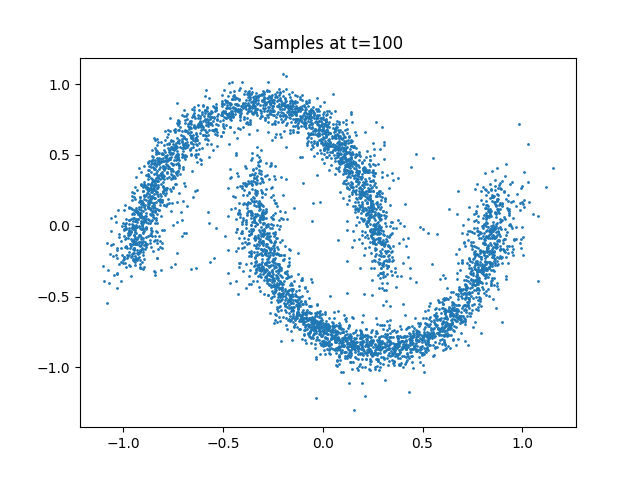
\includegraphics[width=0.3\textwidth]{exps/ddpm_2_100_0.0001_0.02_moons/samples_100.png} \\
        t=10 & t=50 & t=100 \\[0.5em]
        
        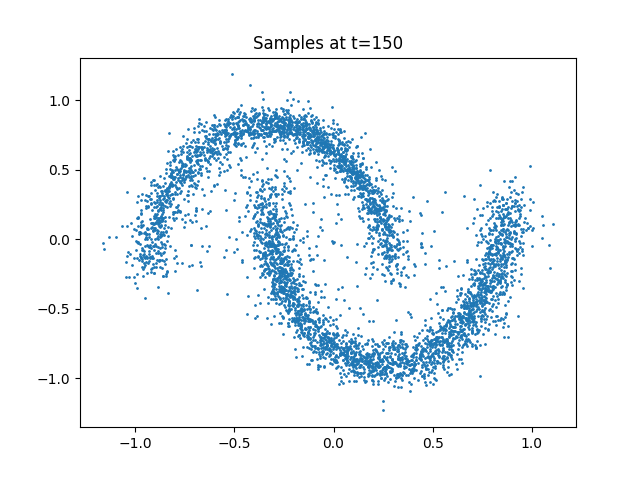
\includegraphics[width=0.3\textwidth]{exps/ddpm_2_150_0.0001_0.02_moons/samples_150.png} &
        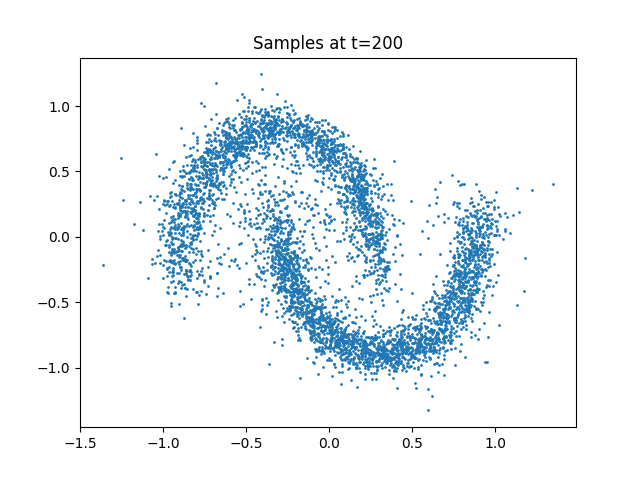
\includegraphics[width=0.3\textwidth]{exps/ddpm_2_200_0.0001_0.02_moons/samples_200.png} &
        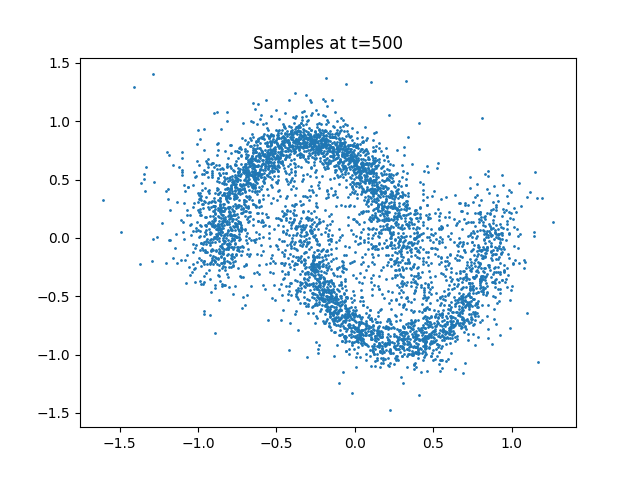
\includegraphics[width=0.3\textwidth]{exps/ddpm_2_500_0.0001_0.02_moons/samples_500.png} \\
        t=150 & t=200 & t=500 \\
    \end{tabular}
    \caption{Samples generated by DDPM with \textbf{varying timesteps} for the Moons dataset.}
    \label{fig:timesteps_moons}
\end{figure}

\begin{figure}[H]
    \centering
    \begin{tabular}{ccc}
        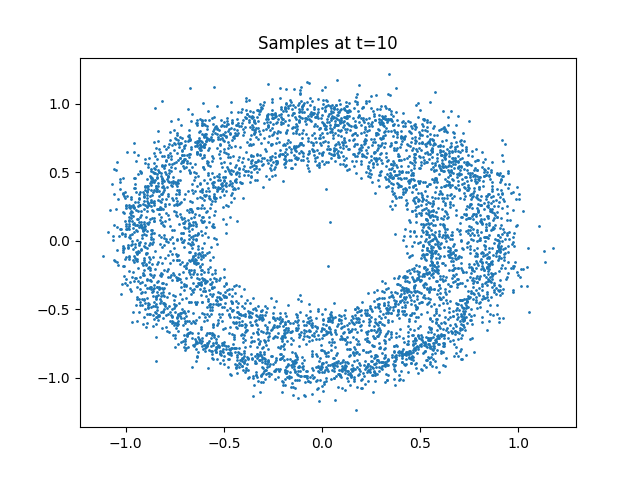
\includegraphics[width=0.3\textwidth]{exps/ddpm_2_10_0.0001_0.02_circles/samples_10.png} &
        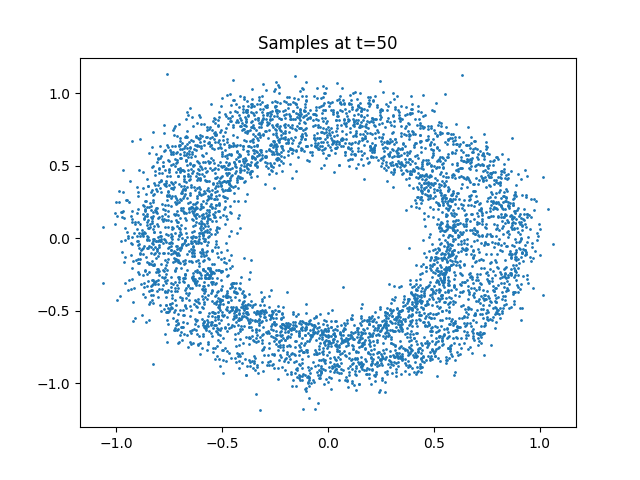
\includegraphics[width=0.3\textwidth]{exps/ddpm_2_50_0.0001_0.02_circles/samples_50.png} &
        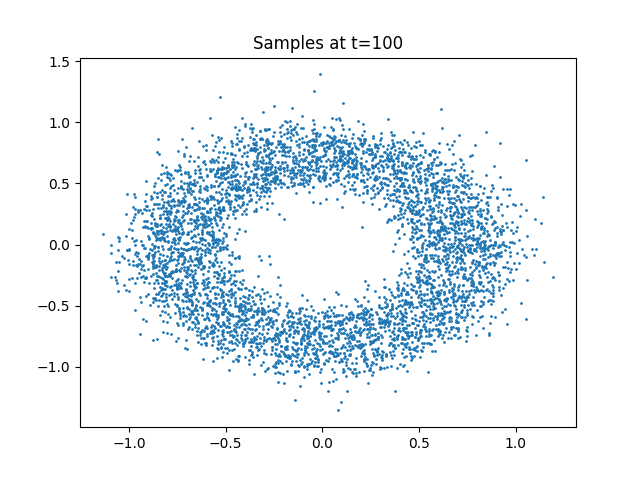
\includegraphics[width=0.3\textwidth]{exps/ddpm_2_100_0.0001_0.02_circles/samples_100.png} \\
        t=10 & t=50 & t=100 \\[0.5em]
        
        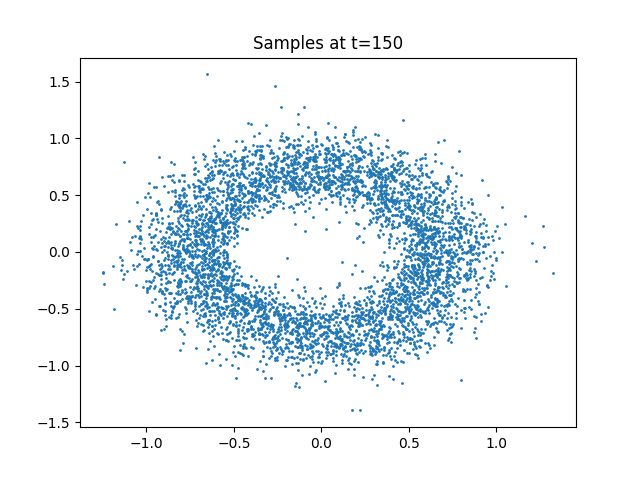
\includegraphics[width=0.3\textwidth]{exps/ddpm_2_150_0.0001_0.02_circles/samples_150.png} &
        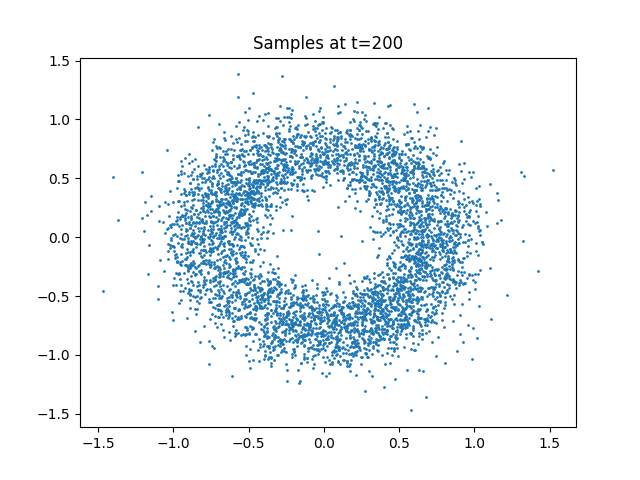
\includegraphics[width=0.3\textwidth]{exps/ddpm_2_200_0.0001_0.02_circles/samples_200.png} &
        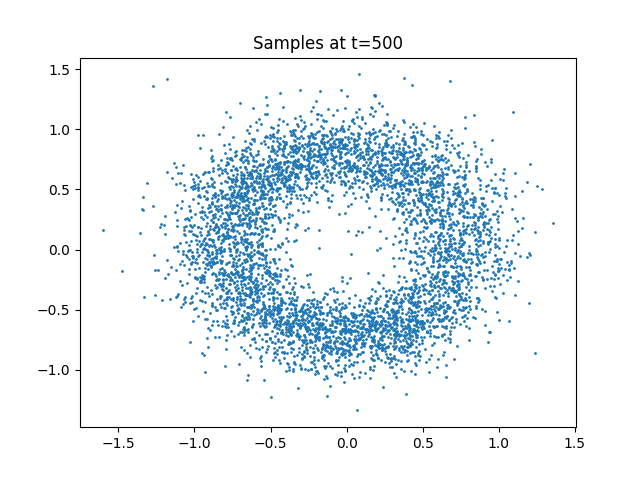
\includegraphics[width=0.3\textwidth]{exps/ddpm_2_500_0.0001_0.02_circles/samples_500.png} \\
        t=150 & t=200 & t=500 \\
    \end{tabular}
    \caption{Samples generated by DDPM with \textbf{varying timesteps} for the Circles dataset.}
    \label{fig:timesteps_circles}
\end{figure}

\begin{figure}[H]
    \centering
    \begin{tabular}{ccc}
        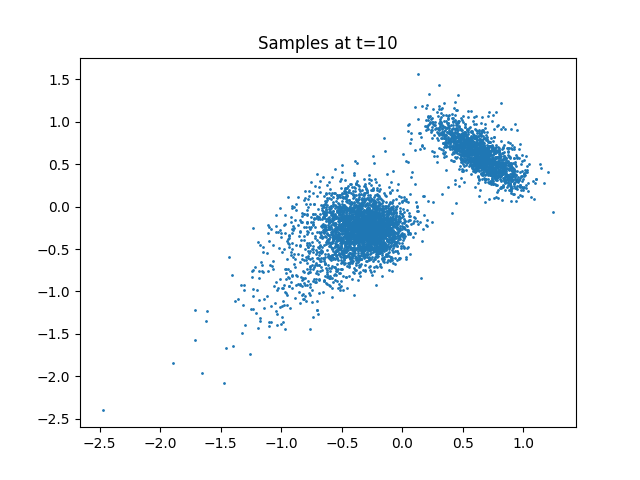
\includegraphics[width=0.3\textwidth]{exps/ddpm_2_10_0.0001_0.02_blobs/samples_10.png} &
        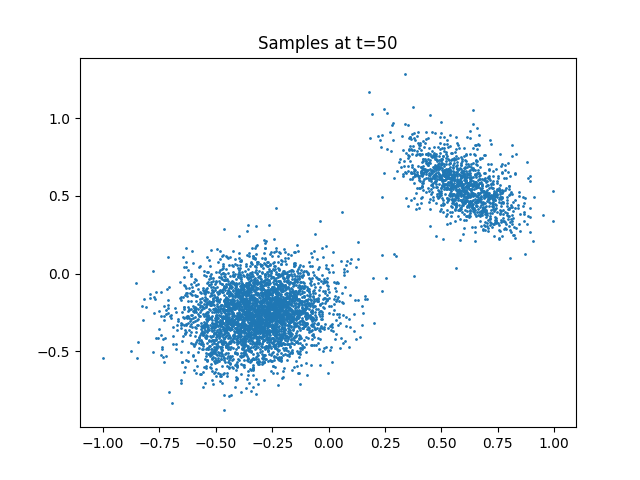
\includegraphics[width=0.3\textwidth]{exps/ddpm_2_50_0.0001_0.02_blobs/samples_50.png} &
        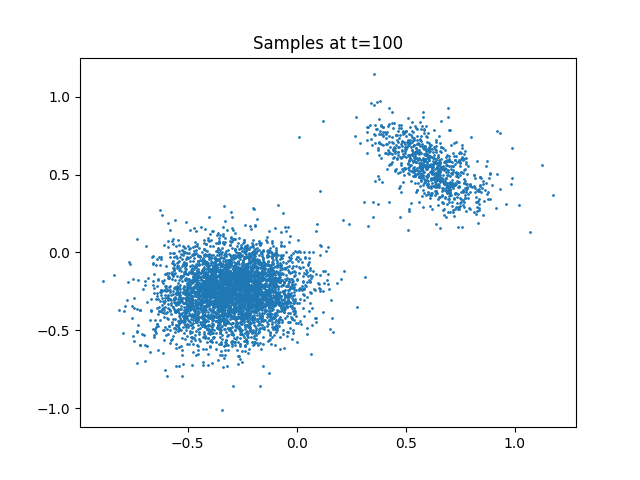
\includegraphics[width=0.3\textwidth]{exps/ddpm_2_100_0.0001_0.02_blobs/samples_100.png} \\
        t=10 & t=50 & t=100 \\[0.5em]
        
        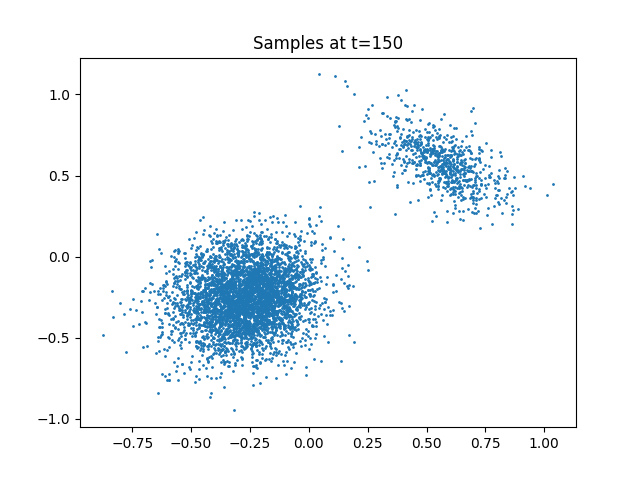
\includegraphics[width=0.3\textwidth]{exps/ddpm_2_150_0.0001_0.02_blobs/samples_150.png} &
        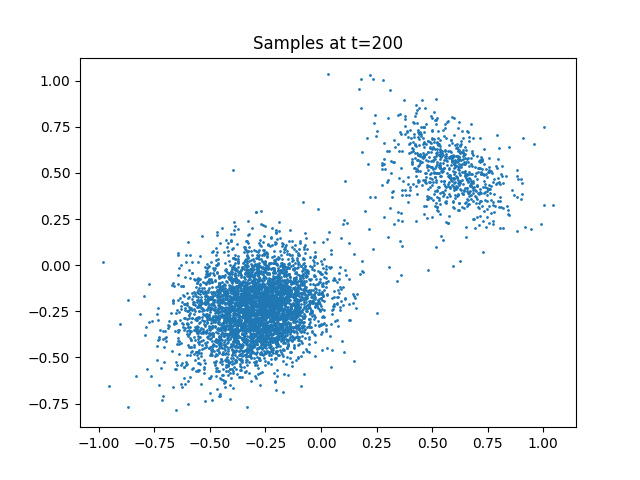
\includegraphics[width=0.3\textwidth]{exps/ddpm_2_200_0.0001_0.02_blobs/samples_200.png} &
        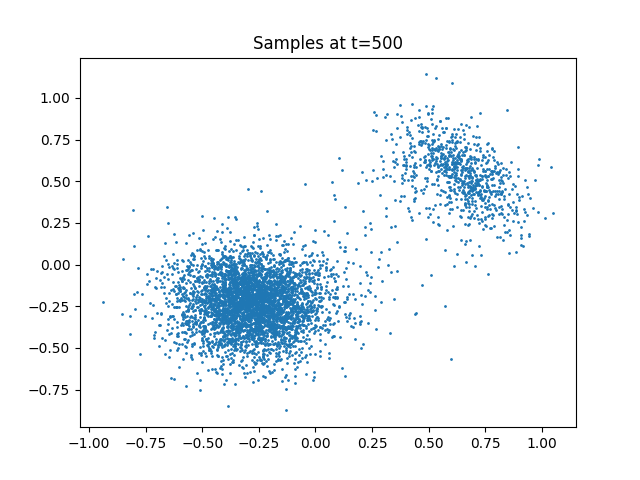
\includegraphics[width=0.3\textwidth]{exps/ddpm_2_500_0.0001_0.02_blobs/samples_500.png} \\
        t=150 & t=200 & t=500 \\
    \end{tabular}
    \caption{Samples generated by DDPM with \textbf{varying timesteps} for the Blobs dataset.}
    \label{fig:timesteps_blobs}
\end{figure}

\begin{figure}[H]
    \centering
    \begin{tabular}{ccc}
        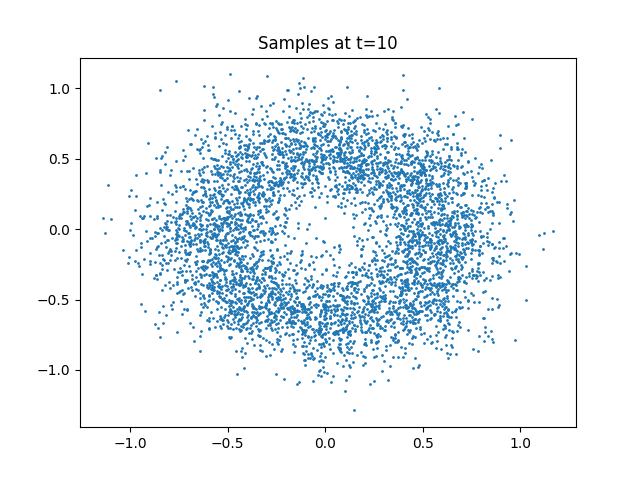
\includegraphics[width=0.3\textwidth]{exps/ddpm_2_10_0.0001_0.02_manycircles/samples_10.png} &
        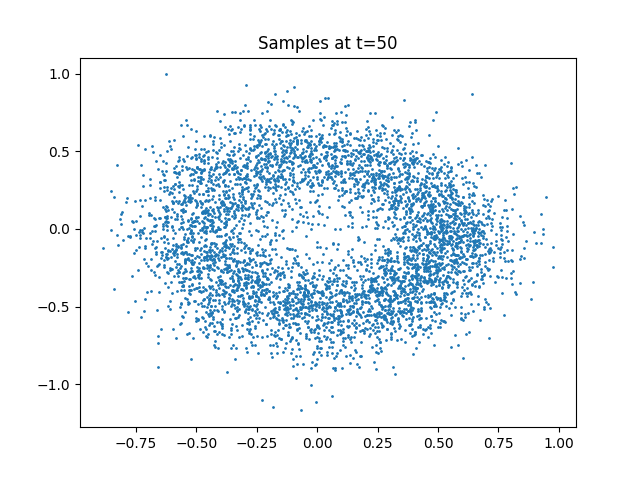
\includegraphics[width=0.3\textwidth]{exps/ddpm_2_50_0.0001_0.02_manycircles/samples_50.png} &
        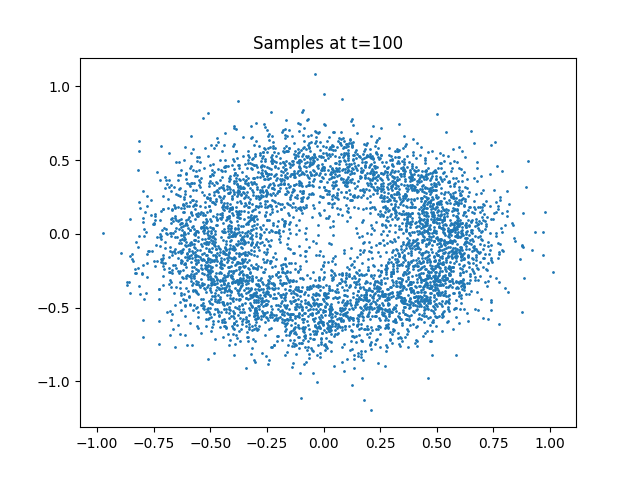
\includegraphics[width=0.3\textwidth]{exps/ddpm_2_100_0.0001_0.02_manycircles/samples_100.png} \\
        t=10 & t=50 & t=100 \\[0.5em]
        
        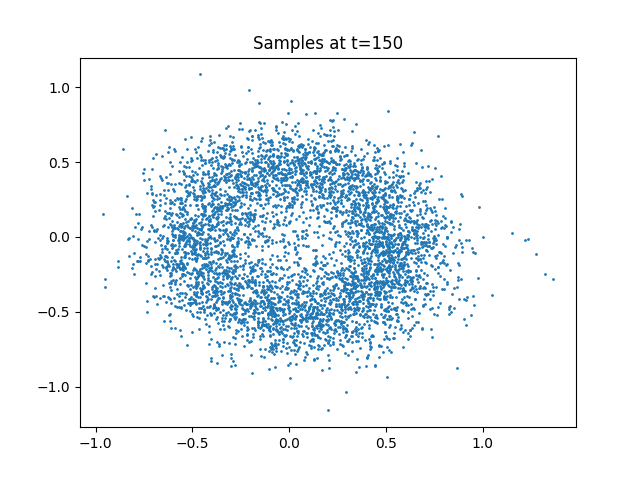
\includegraphics[width=0.3\textwidth]{exps/ddpm_2_150_0.0001_0.02_manycircles/samples_150.png} &
        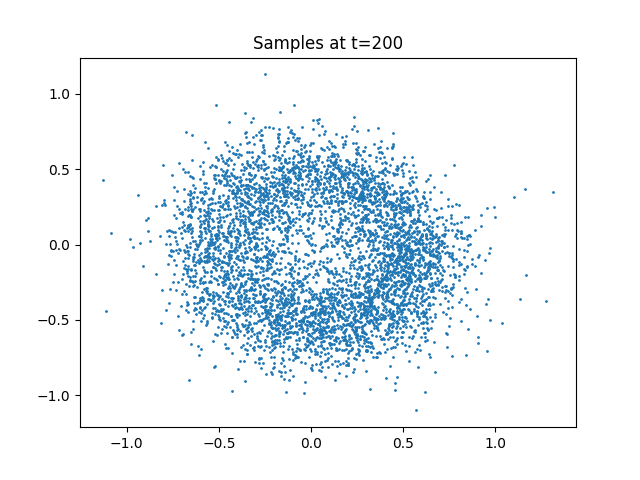
\includegraphics[width=0.3\textwidth]{exps/ddpm_2_200_0.0001_0.02_manycircles/samples_200.png} &
        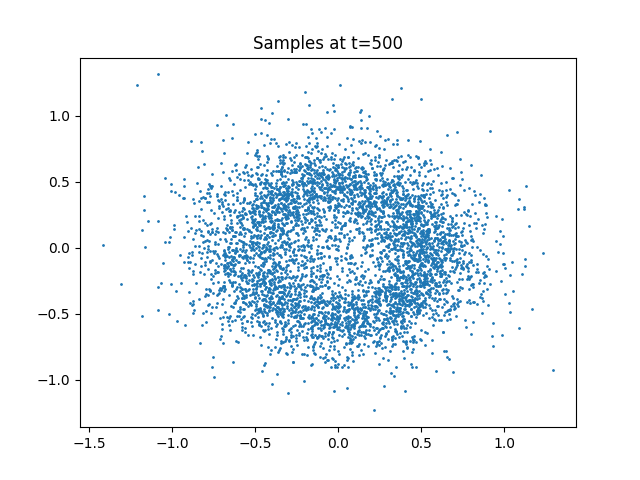
\includegraphics[width=0.3\textwidth]{exps/ddpm_2_500_0.0001_0.02_manycircles/samples_500.png} \\
        t=150 & t=200 & t=500 \\
    \end{tabular}
    \caption{Samples generated by DDPM with \textbf{varying timesteps} for the Manycircles dataset.}
    \label{fig:timesteps_manycircles}
\end{figure}

\begin{figure}[H]
    \centering
    \begin{tabular}{ccc}
        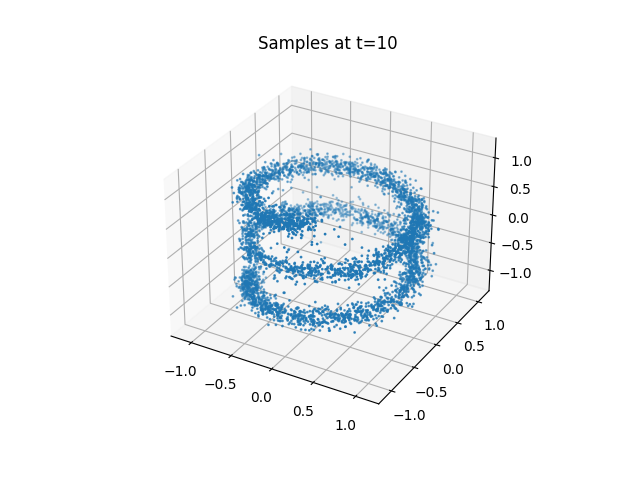
\includegraphics[width=0.3\textwidth]{exps/ddpm_3_10_0.0001_0.02_helix/samples_10.png} &
        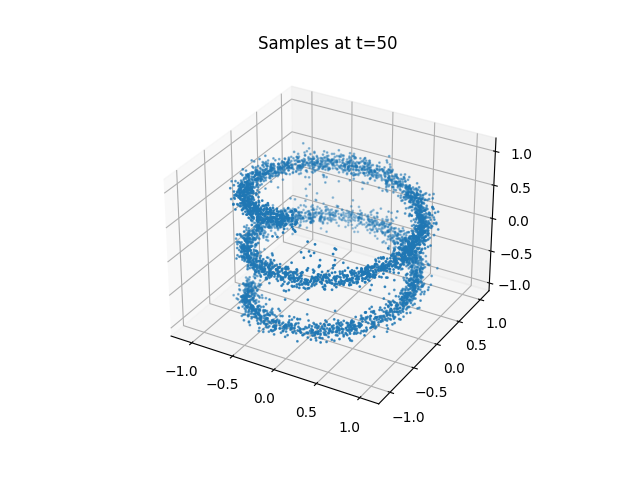
\includegraphics[width=0.3\textwidth]{exps/ddpm_3_50_0.0001_0.02_helix/samples_50.png} &
        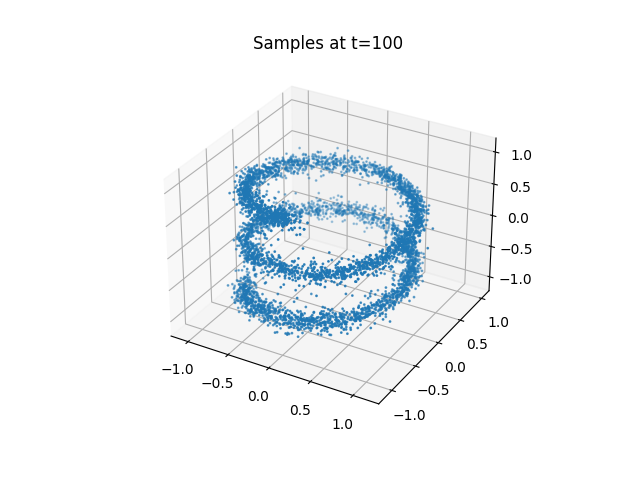
\includegraphics[width=0.3\textwidth]{exps/ddpm_3_100_0.0001_0.02_helix/samples_100.png} \\
        t=10 & t=50 & t=100 \\[0.5em]
        
        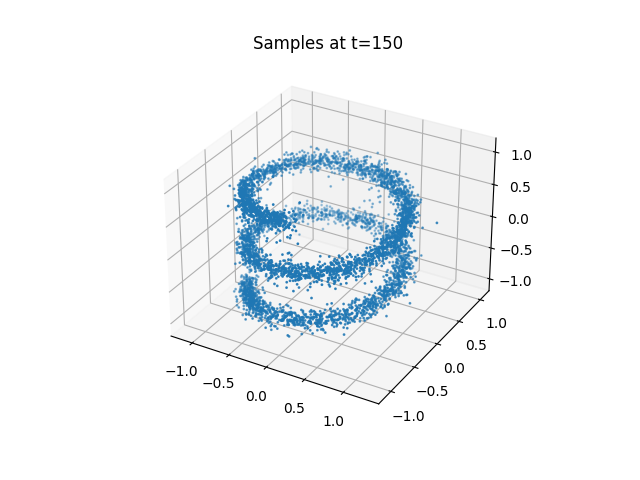
\includegraphics[width=0.3\textwidth]{exps/ddpm_3_150_0.0001_0.02_helix/samples_150.png} &
        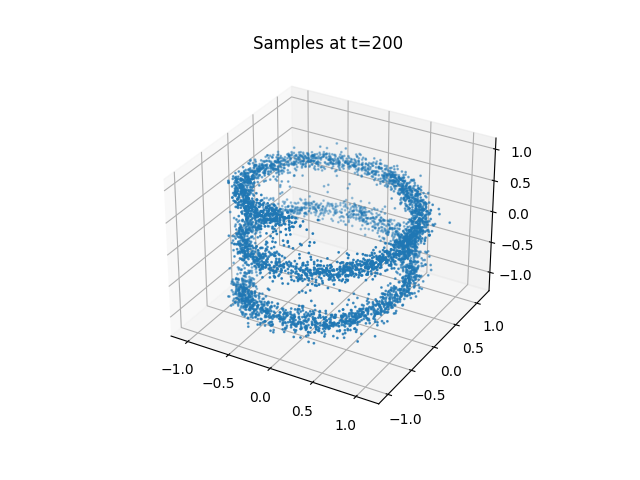
\includegraphics[width=0.3\textwidth]{exps/ddpm_3_200_0.0001_0.02_helix/samples_200.png} &
        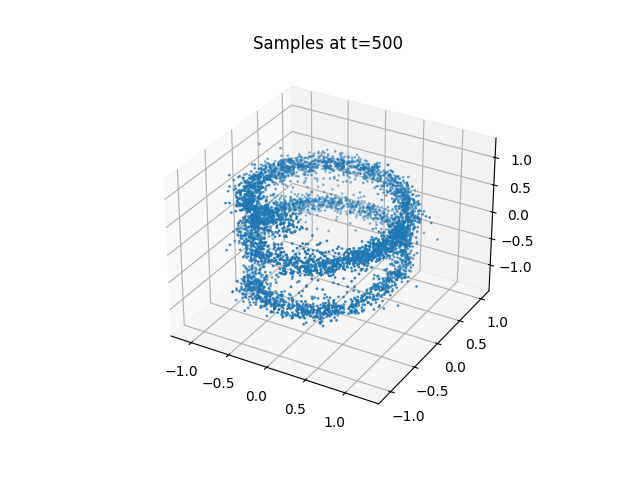
\includegraphics[width=0.3\textwidth]{exps/ddpm_3_500_0.0001_0.02_helix/samples_500.png} \\
        t=150 & t=200 & t=500 \\
    \end{tabular}
    \caption{Samples generated by DDPM with \textbf{varying timesteps} for the Helix dataset.}
    \label{fig:timesteps_helix}
\end{figure}

\subsubsection{Varying Beta Schedule}
Here, timesteps = 200.

\begin{longtable}{|l|l|c|c|c|c|c|c|}
    \hline
     \textbf{Dataset} & \textbf{Metric} & \multicolumn{6}{c|}{\textbf{Beta Schedule (lbeta→ubeta)}} \\
     \cline{3-8}
     & & \textbf{1e-4→0.02} & \textbf{1e-3→0.2} & \textbf{1e-5→0.002} & \textbf{1e-5→0.02} & \textbf{1e-4→0.2} & \textbf{1e-5→0.2} \\
    \hline
        \multirow{2}{*}{Moons} & EMD & 30.55 & 35.57 & 34.76 & \textbf{30.48} & 33.48 & 33.62 \\
        \cline{2-8}
        & NLL & 0.94 & \textbf{0.93} & 0.98 & 0.95 & 0.95 & 0.94 \\
        \hline
        \multirow{2}{*}{Circles} & EMD & 38.62 & 38.03 & \textbf{33.03} & 38.36 & 36.52 & 37.45 \\
        \cline{2-8}
        & NLL & 1.01 & \textbf{1.00} & 1.02 & \textbf{1.00} & 1.01 & 1.01 \\
        \hline
        \multirow{2}{*}{Blobs} & EMD & \textbf{17.17} & 20.35 & 62.98 & \textbf{17.17} & 19.59 & 19.62 \\
        \cline{2-8}
        & NLL & 0.01 & 0.02 & 0.20 & 0.01 & 0.01 & \textbf{0.00} \\
        \hline
        \multirow{2}{*}{Manycircles} & EMD & 30.98 & 28.75 & \textbf{26.55} & 31.82 & 29.40 & 29.92 \\
        \cline{2-8}
        & NLL & 0.54 & \textbf{0.52} & 0.58 & 0.53 & 0.53 & 0.54 \\
        \hline
        \multirow{2}{*}{Helix} & EMD & 58.87 & \textbf{56.25} & 57.31 & 58.29 & 57.34 & 58.72 \\
        \cline{2-8}
        & NLL & 1.53 & \textbf{1.52} & 1.54 & 1.53 & 1.53 & 1.52 \\
        \hline
        \caption{EMD and NLL values for DDPM with varying beta schedules.}
\end{longtable}

For the beta schedule comparison, there isn't a single schedule that works universally best across all datasets. However, there are some general trends:

\begin{itemize}
    \item For Moons dataset: 1e-5→0.02 works best for EMD (30.48)
    \item For Circles dataset: 1e-5→0.002 works best for EMD (33.03)
    \item For Blobs dataset: 1e-4→0.02 and 1e-5→0.02 work best for EMD (17.17)
    \item For Manycircles dataset: 1e-5→0.002 works best for EMD (26.55)
    \item For Helix dataset: 1e-3→0.2 works best for EMD (56.25)
\end{itemize}

For NLL metrics, slightly higher upper beta values tend to work better, with 1e-3→0.2 achieving the best NLL for several datasets.


\begin{figure}[H]
    \centering
    \begin{tabular}{ccc}
        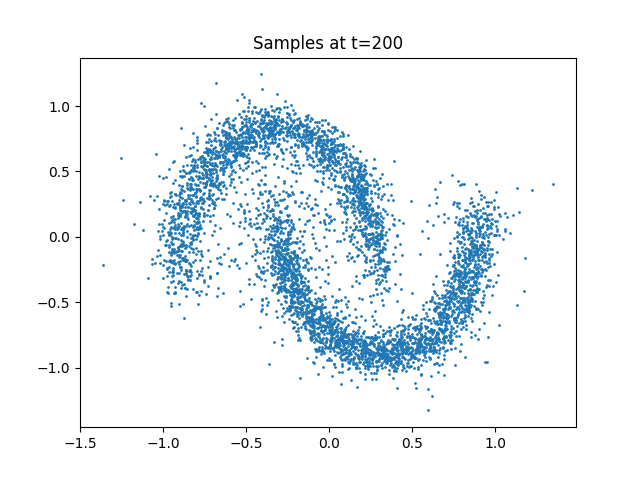
\includegraphics[width=0.3\textwidth]{exps/ddpm_2_200_0.0001_0.02_moons/samples_200.png} &
        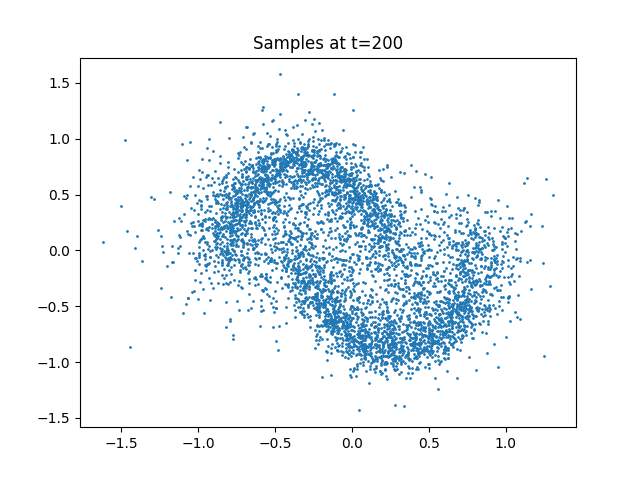
\includegraphics[width=0.3\textwidth]{exps/ddpm_2_200_0.001_0.2_moons/samples_200.png} &
        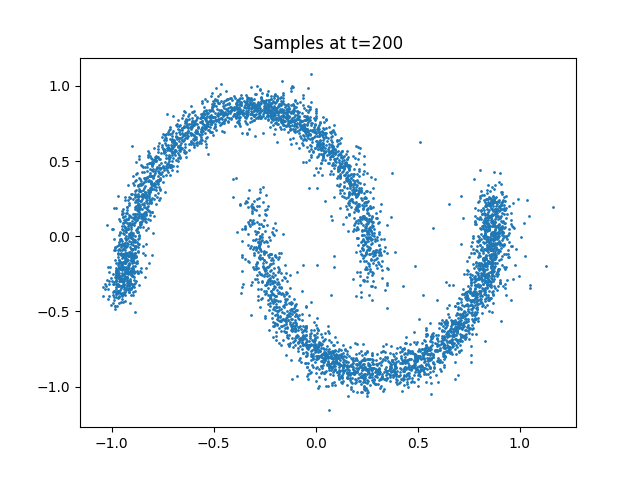
\includegraphics[width=0.3\textwidth]{exps/ddpm_2_200_1e-05_0.002_moons/samples_200.png} \\
        $\beta=1\text{e-}4\to0.02$ & $\beta=1\text{e-}3\to0.2$ & $\beta=1\text{e-}5\to0.002$ \\[0.5em]
        
        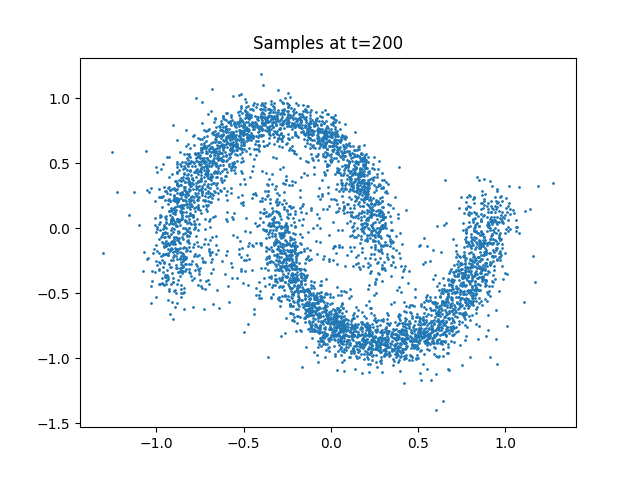
\includegraphics[width=0.3\textwidth]{exps/ddpm_2_200_1e-05_0.02_moons/samples_200.png} &
        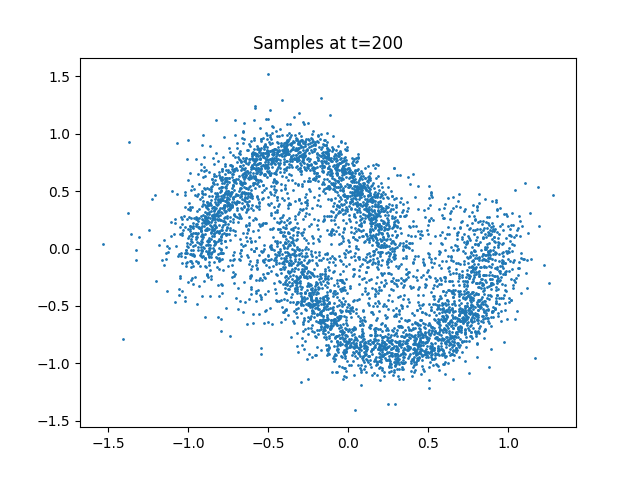
\includegraphics[width=0.3\textwidth]{exps/ddpm_2_200_0.0001_0.2_moons/samples_200.png} &
        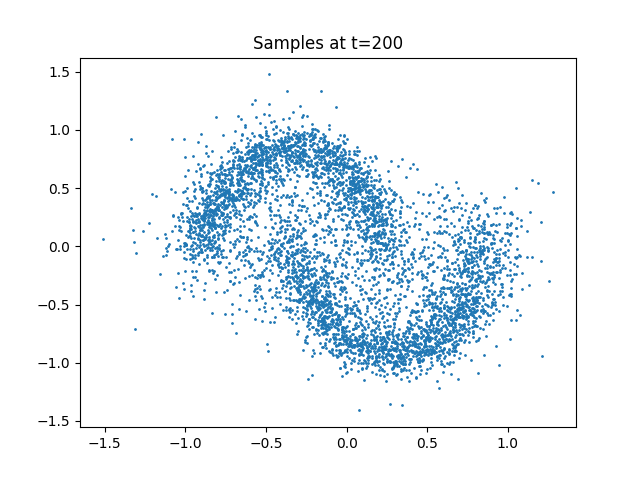
\includegraphics[width=0.3\textwidth]{exps/ddpm_2_200_1e-05_0.2_moons/samples_200.png} \\
        $\beta=1\text{e-}5\to0.02$ & $\beta=1\text{e-}4\to0.2$ & $\beta=1\text{e-}5\to0.2$ \\
    \end{tabular}
    \caption{Samples generated by DDPM with \textbf{varying beta schedules} for the Moons dataset.}
    \label{fig:beta_moons}
\end{figure}

\begin{figure}[H]
    \centering
    \begin{tabular}{ccc}
        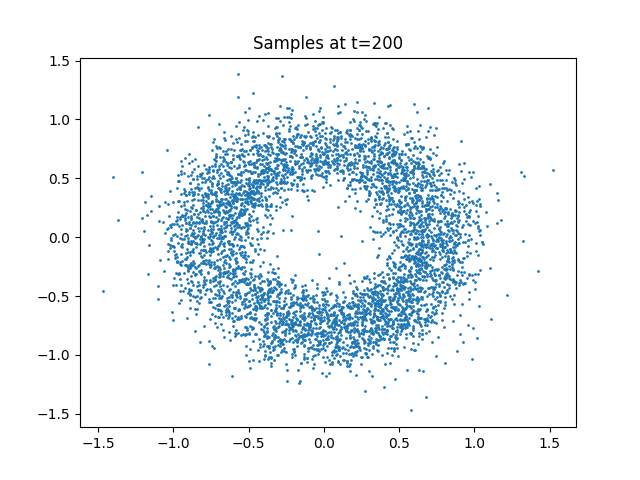
\includegraphics[width=0.3\textwidth]{exps/ddpm_2_200_0.0001_0.02_circles/samples_200.png} &
        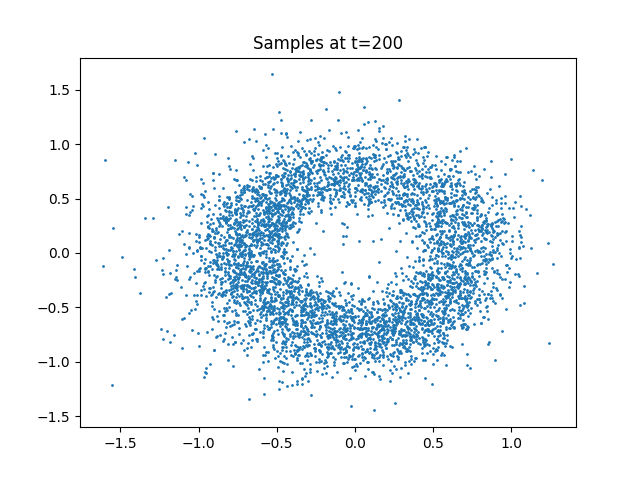
\includegraphics[width=0.3\textwidth]{exps/ddpm_2_200_0.001_0.2_circles/samples_200.png} &
        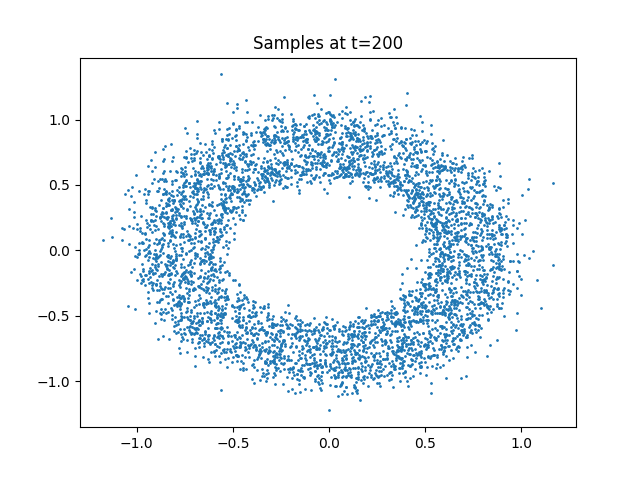
\includegraphics[width=0.3\textwidth]{exps/ddpm_2_200_1e-05_0.002_circles/samples_200.png} \\
        $\beta=1\text{e-}4\to0.02$ & $\beta=1\text{e-}3\to0.2$ & $\beta=1\text{e-}5\to0.002$ \\[0.5em]
        
        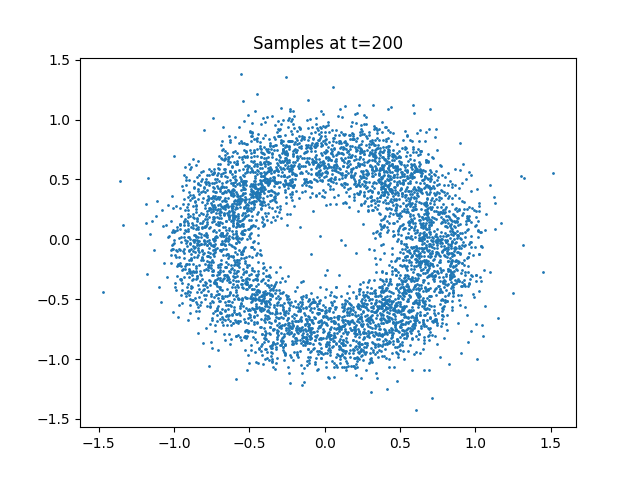
\includegraphics[width=0.3\textwidth]{exps/ddpm_2_200_1e-05_0.02_circles/samples_200.png} &
        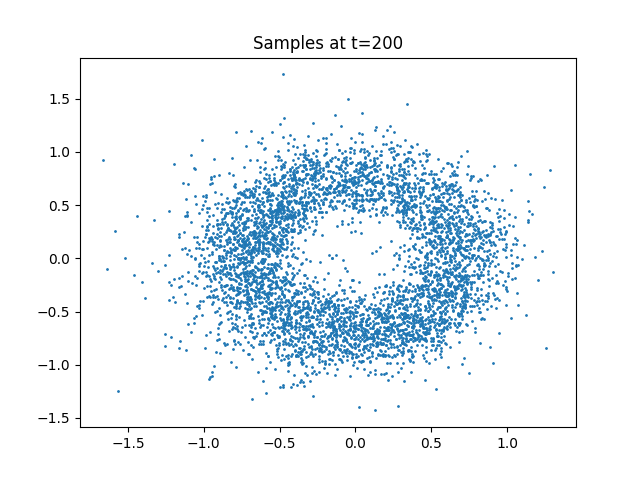
\includegraphics[width=0.3\textwidth]{exps/ddpm_2_200_0.0001_0.2_circles/samples_200.png} &
        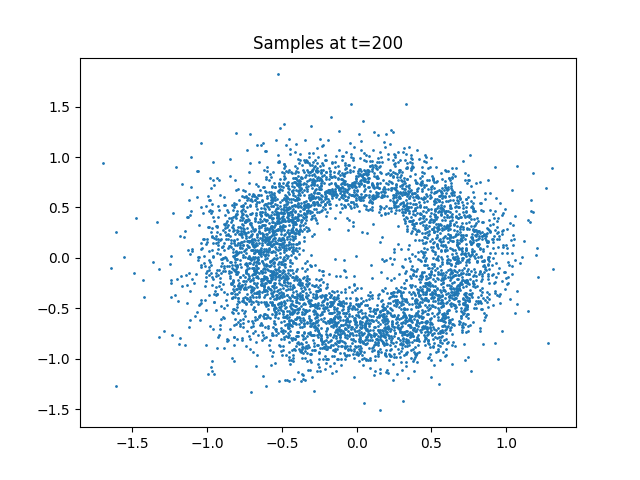
\includegraphics[width=0.3\textwidth]{exps/ddpm_2_200_1e-05_0.2_circles/samples_200.png} \\
        $\beta=1\text{e-}5\to0.02$ & $\beta=1\text{e-}4\to0.2$ & $\beta=1\text{e-}5\to0.2$ \\
    \end{tabular}
    \caption{Samples generated by DDPM with \textbf{varying beta schedules} for the Circles dataset.}
    \label{fig:beta_circles}
\end{figure}

\begin{figure}[H]
    \centering
    \begin{tabular}{ccc}
        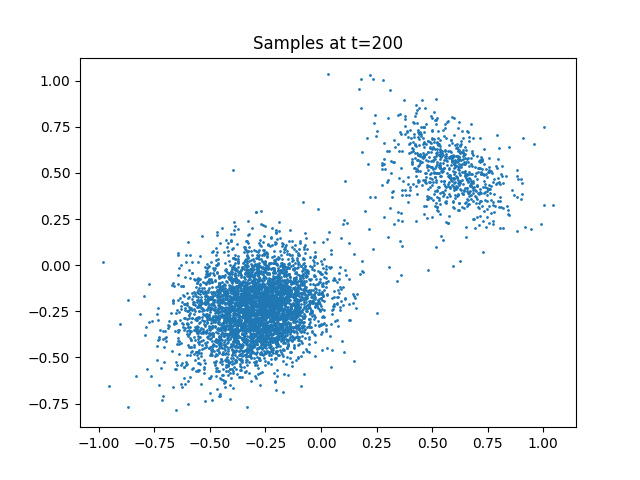
\includegraphics[width=0.3\textwidth]{exps/ddpm_2_200_0.0001_0.02_blobs/samples_200.png} &
        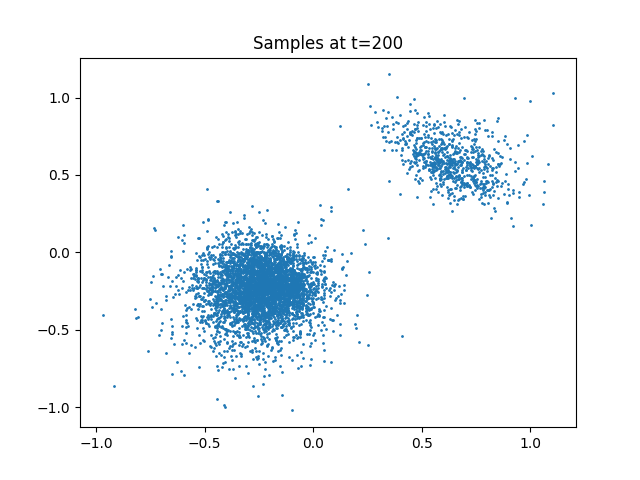
\includegraphics[width=0.3\textwidth]{exps/ddpm_2_200_0.001_0.2_blobs/samples_200.png} &
        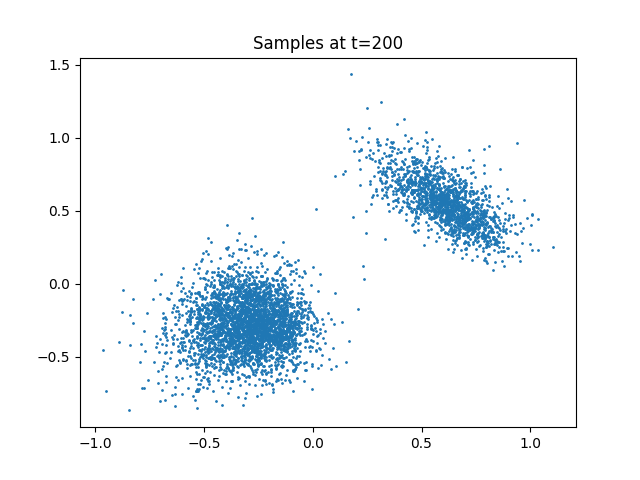
\includegraphics[width=0.3\textwidth]{exps/ddpm_2_200_1e-05_0.002_blobs/samples_200.png} \\
        $\beta=1\text{e-}4\to0.02$ & $\beta=1\text{e-}3\to0.2$ & $\beta=1\text{e-}5\to0.002$ \\[0.5em]
        
        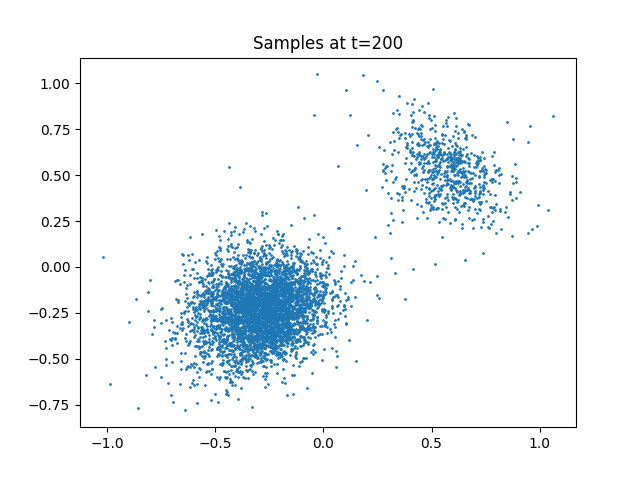
\includegraphics[width=0.3\textwidth]{exps/ddpm_2_200_1e-05_0.02_blobs/samples_200.png} &
        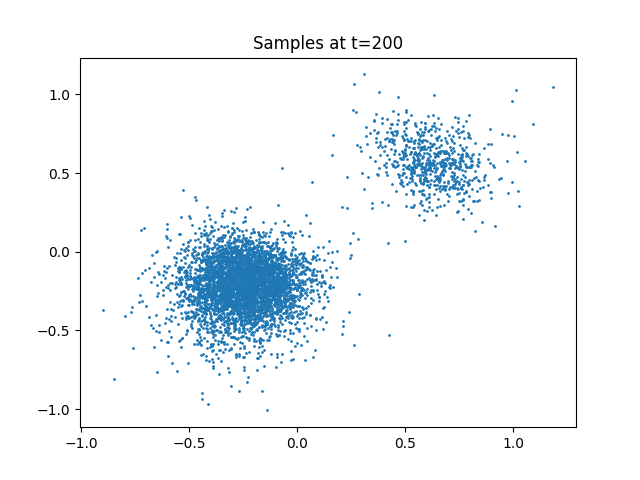
\includegraphics[width=0.3\textwidth]{exps/ddpm_2_200_0.0001_0.2_blobs/samples_200.png} &
        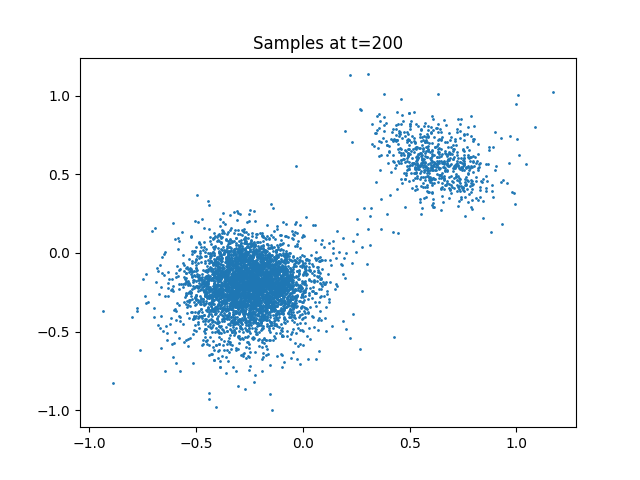
\includegraphics[width=0.3\textwidth]{exps/ddpm_2_200_1e-05_0.2_blobs/samples_200.png} \\
        $\beta=1\text{e-}5\to0.02$ & $\beta=1\text{e-}4\to0.2$ & $\beta=1\text{e-}5\to0.2$ \\
    \end{tabular}
    \caption{Samples generated by DDPM with \textbf{varying beta schedules} for the Blobs dataset.}
    \label{fig:beta_blobs}
\end{figure}

\begin{figure}[H]
    \centering
    \begin{tabular}{ccc}
        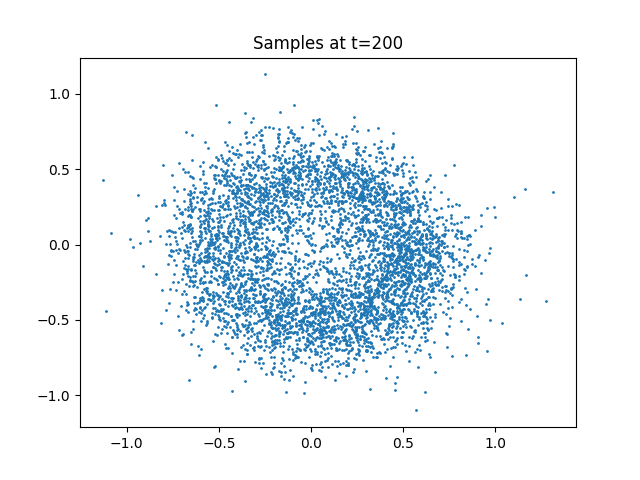
\includegraphics[width=0.3\textwidth]{exps/ddpm_2_200_0.0001_0.02_manycircles/samples_200.png} &
        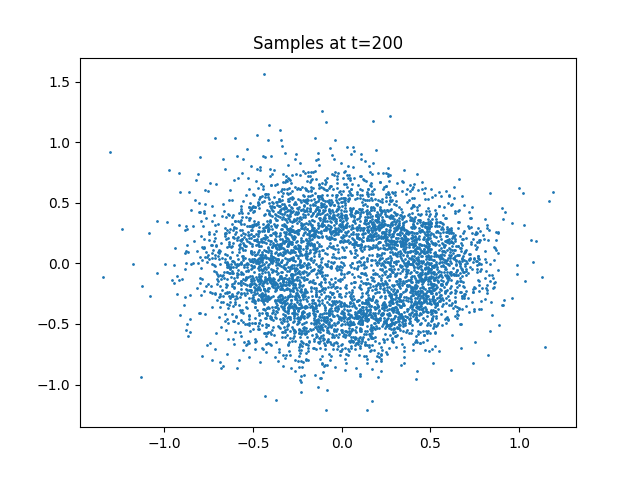
\includegraphics[width=0.3\textwidth]{exps/ddpm_2_200_0.001_0.2_manycircles/samples_200.png} &
        \includegraphics[width=0.3\textwidth]{exps/ddpm_2_200_1e-05_0.002_manycircles/samples_200.png} \\
        $\beta=1\text{e-}4\to0.02$ & $\beta=1\text{e-}3\to0.2$ & $\beta=1\text{e-}5\to0.002$ \\[0.5em]
        
        \includegraphics[width=0.3\textwidth]{exps/ddpm_2_200_1e-05_0.02_manycircles/samples_200.png} &
        \includegraphics[width=0.3\textwidth]{exps/ddpm_2_200_0.0001_0.2_manycircles/samples_200.png} &
        \includegraphics[width=0.3\textwidth]{exps/ddpm_2_200_1e-05_0.2_manycircles/samples_200.png} \\
        $\beta=1\text{e-}5\to0.02$ & $\beta=1\text{e-}4\to0.2$ & $\beta=1\text{e-}5\to0.2$ \\
    \end{tabular}
    \caption{Samples generated by DDPM with \textbf{varying beta schedules} for the Manycircles dataset.}
    \label{fig:beta_manycircles}
\end{figure}

\begin{figure}[H]
    \centering
    \begin{tabular}{ccc}
        \includegraphics[width=0.3\textwidth]{exps/ddpm_3_200_0.0001_0.02_helix/samples_200.png} &
        \includegraphics[width=0.3\textwidth]{exps/ddpm_3_200_0.001_0.2_helix/samples_200.png} &
        \includegraphics[width=0.3\textwidth]{exps/ddpm_3_200_1e-05_0.002_helix/samples_200.png} \\
        $\beta=1\text{e-}4\to0.02$ & $\beta=1\text{e-}3\to0.2$ & $\beta=1\text{e-}5\to0.002$ \\[0.5em]
        
        \includegraphics[width=0.3\textwidth]{exps/ddpm_3_200_1e-05_0.02_helix/samples_200.png} &
        \includegraphics[width=0.3\textwidth]{exps/ddpm_3_200_0.0001_0.2_helix/samples_200.png} &
        \includegraphics[width=0.3\textwidth]{exps/ddpm_3_200_1e-05_0.2_helix/samples_200.png} \\
        $\beta=1\text{e-}5\to0.02$ & $\beta=1\text{e-}4\to0.2$ & $\beta=1\text{e-}5\to0.2$ \\
    \end{tabular}
    \caption{Samples generated by DDPM with \textbf{varying beta schedules} for the Helix dataset.}
    \label{fig:beta_helix}
\end{figure}

\newpage

\subsubsection{Cosine and Sigmoid schedules}
Here, timesteps = 200.
\begin{longtable}{|l|l|c|c|}
    \hline
     \textbf{Dataset} & \textbf{Metric} & \multicolumn{2}{c|}{\textbf{Schedule}} \\
     \cline{3-4}
     & & \textbf{Cosine} & \textbf{Sigmoid} \\
    \hline
        \multirow{2}{*}{Moons} & EMD & \textbf{28.29} & 30.88 \\
        \cline{2-4}
        & NLL & 0.96 & \textbf{0.93} \\
        \hline
        \multirow{2}{*}{Circles} & EMD & \textbf{39.77} & 41.68 \\
        \cline{2-4}
        & NLL & \textbf{1.01} & 1.02 \\
        \hline
        \multirow{2}{*}{Blobs} & EMD & 15.54 & \textbf{15.18} \\
        \cline{2-4}
        & NLL & \textbf{0.00} & \textbf{0.00} \\
        \hline
        \multirow{2}{*}{Manycircles} & EMD & \textbf{30.80} & 33.37 \\
        \cline{2-4}
        & NLL & 0.54 & \textbf{0.53} \\
        \hline
        \multirow{2}{*}{Helix} & EMD & 56.88 & \textbf{54.38} \\
        \cline{2-4}
        & NLL & \textbf{1.54} & \textbf{1.54} \\
        \hline
        \caption{EMD and NLL values for DDPM with cosine and sigmoid schedules.}
\end{longtable}


\begin{figure}[H]
    \centering
    \begin{tabular}{ccc}
        \includegraphics[width=0.3\textwidth]{exps/ddpm_2_200_cosine_moons/samples_200.png} &
        \includegraphics[width=0.3\textwidth]{exps/ddpm_2_200_cosine_circles/samples_200.png} &
        \includegraphics[width=0.3\textwidth]{exps/ddpm_2_200_cosine_blobs/samples_200.png} \\
        Moons & Circles & Blobs \\[0.5em]
        
        \includegraphics[width=0.3 \textwidth]{exps/ddpm_2_200_cosine_manycircles/samples_200.png} &
        \includegraphics[width=0.3\textwidth]{exps/ddpm_3_200_cosine_helix/samples_200.png} & \\
        Manycircles & Helix & \\
    \end{tabular}
    \caption{Samples generated by DDPM with \textbf{cosine schedule} for various datasets.}
    \label{fig:cosine_schedule}
\end{figure}

\begin{figure}[H]
    \centering
    \begin{tabular}{ccc}
        \includegraphics[width=0.3\textwidth]{exps/ddpm_2_200_sigmoid_moons/samples_200.png} &
        \includegraphics[width=0.3\textwidth]{exps/ddpm_2_200_sigmoid_circles/samples_200.png} &
        \includegraphics[width=0.3\textwidth]{exps/ddpm_2_200_sigmoid_blobs/samples_200.png} \\
        Moons & Circles & Blobs \\[0.5em]
        
        \includegraphics[width=0.3\textwidth]{exps/ddpm_2_200_sigmoid_manycircles/samples_200.png} &
        \includegraphics[width=0.3\textwidth]{exps/ddpm_3_200_sigmoid_helix/samples_200.png} & \\
        Manycircles & Helix & \\
    \end{tabular}
    \caption{Samples generated by DDPM with \textbf{sigmoid schedule} for various datasets.}
    \label{fig:sigmoid_schedule}
\end{figure}

\subsubsection{Training Albatross}
The hyperparameters used for training Albatross are as follows:
\begin{itemize}
    \item \textbf{Timesteps}: 150
    \item \textbf{Beta Schedule}: 1e-4→0.02
\end{itemize}

\section{Classifier-Free Guidance}

For EMD calculation, the number of subsamples is set to 250 and the number of iterations is set to 5.

For all training runs, the hyperparameters used are as follows:
\begin{itemize}
    \item \textbf{Epochs}: 100
    \item \textbf{Batch Size}: 64
    \item \textbf{Learning Rate}: 1e-3
    \item \textbf{Number of Samples}: 20000
    \item \textbf{lbeta}: 0.0001
    \item \textbf{ubeta}: 0.02
    \item \textbf{p\_uncond} (required for CFG training): 0.2
\end{itemize}

\subsection{Guided vs. Conditional Sampling}

\begin{itemize}
    \item \textbf{Training:} Conditional sampling requires the model to be trained with explicit labels, while guided sampling can work even with an unconditional model.
    
    \item \textbf{Control:} Conditional sampling directly conditions the model on labels, whereas guided sampling modifies the noise prediction using a guidance scale.
    
    \item \textbf{Flexibility:} Conditional sampling is fixed after training, while guided sampling allows dynamic tuning of the guidance strength during inference.
    
    \item \textbf{Diversity:} Conditional sampling maintains diversity in generated samples, but guided sampling can reduce diversity if the guidance scale is too high.
    
    \item \textbf{Best Use Case:} Conditional sampling is ideal when training a model from scratch, while guided sampling is useful when modifying an already trained model.
\end{itemize}

\subsection{Architecture}

The model architecture for Classifier-Free Guidance (CFG) is similar to DDPM, with the modification of concatenating a class embedding to the input layer. The class embedding is a sinusoidal position embedding similar to the time embedding used in DDPM.

\subsection{Unguided Conditional DDPM Results}

\begin{figure}[H]
    \centering
    \begin{tabular}{ccc}
        \includegraphics[width=0.3\textwidth]{exps/ddpm_2_150_0.0001_0.02_moons/samples_conditional_150.png} &
        \includegraphics[width=0.3\textwidth]{exps/ddpm_2_150_0.0001_0.02_circles/samples_conditional_150.png} &
        \includegraphics[width=0.3\textwidth]{exps/ddpm_2_150_0.0001_0.02_blobs/samples_conditional_150.png} \\
        Moons & Circles & Blobs \\[0.5em]
        
        
        \includegraphics[width=0.3\textwidth]{exps/ddpm_2_150_0.0001_0.02_manycircles/samples_conditional_150.png} &
        \includegraphics[width=0.3\textwidth]{exps/ddpm_3_150_0.0001_0.02_helix/samples_conditional_150.png} & \\
        Manycircles & Helix & \\
    \end{tabular}
    \caption{Samples generated by \textbf{conditional} DDPM for various datasets.}
    \label{fig:cond_all_data}
\end{figure}

\newpage

\subsection{Classifier-Free Guidance Results}

\begin{longtable}{|l|l|c|c|c|c|c|}
    \hline
    \textbf{Dataset} & \textbf{Metric} & \multicolumn{5}{c|}{\textbf{Guidance Scale}} \\
    \cline{3-7}
    & & \textbf{0.25} & \textbf{0.5} & \textbf{1.0} & \textbf{2.0} & \textbf{4.0} \\
    \hline
    \multirow{2}{*}{Moons} & EMD & \textbf{27.23} & 31.77 & 44.57 & 63.59 & 82.62 \\
    \cline{2-7}
    & Accuracy & \textbf{1.00} & \textbf{1.00} & \textbf{1.00} & \textbf{1.00} & \textbf{1.00} \\
    \hline
    \multirow{2}{*}{Circles} & EMD & 40.60 & \textbf{40.33} & 40.65 & 42.87 & 56.30 \\
    \cline{2-7}
    & Accuracy & 0.97 & 0.99 & \textbf{1.00} & \textbf{1.00} & \textbf{1.00} \\
    \hline
    \multirow{2}{*}{Blobs} & EMD & \textbf{20.27} & 26.16 & 39.27 & 55.48 & 77.69 \\
    \cline{2-7}
    & Accuracy & 0.95 & 0.98 & 0.99 & \textbf{1.00} & \textbf{1.00} \\
    \hline
    \multirow{2}{*}{Manycircles} & EMD & \textbf{12.16} & 14.62 & 18.97 & 25.14 & 34.04 \\
    \cline{2-7}
    & Accuracy & 0.92 & 0.96 & 0.98 & \textbf{1.00} & \textbf{1.00} \\
    \hline
    \multirow{2}{*}{Helix} & EMD & \textbf{56.82} & 58.13 & 63.17 & 74.67 & 97.19 \\
    \cline{2-7}
    & Accuracy & 0.73 & 0.76 & 0.82 & 0.88 & \textbf{0.94} \\
    \hline
    \caption{EMD and accuracy values for CFG with varying guidance scales.}
\end{longtable}
\label{tab:cfg_results}

Earth Mover's Distance (EMD) is used because it measures the minimum cost to transform one distribution into another, accounting for geometric relationships between points. EMD evaluates the entire distribution, effectively capturing how well generated samples match the true data.

We observe a clear trade-off between sample quality (measured by EMD) and conditional accuracy across all datasets. As the guidance scale increases, the accuracy generally improves. However, this comes at the cost of increasing EMD values, suggesting that the generated samples may stray further from the true data distribution.

\begin{figure}[H]
    \centering
    \begin{tabular}{ccc}
        \includegraphics[width=0.3\textwidth]{exps/ddpm_2_150_0.0001_0.02_moons/samples_cfg_150_0.25.png} &
        \includegraphics[width=0.3\textwidth]{exps/ddpm_2_150_0.0001_0.02_moons/samples_cfg_150_0.5.png} &
        \includegraphics[width=0.3\textwidth]{exps/ddpm_2_150_0.0001_0.02_moons/samples_cfg_150_1.0.png} \\
        guidance=0.25 & guidance=0.5 & guidance=1.0 \\ [0.5em]

        \includegraphics[width=0.3\textwidth]{exps/ddpm_2_150_0.0001_0.02_moons/samples_cfg_150_2.0.png} &
        \includegraphics[width=0.3\textwidth]{exps/ddpm_2_150_0.0001_0.02_moons/samples_cfg_150_4.0.png} & \\
        guidance=2.0 & guidance=4.0 & \\
    \end{tabular}
    \caption{Samples generated by DDPM with \textbf{varying guidance scales} for the Moons dataset.}
    \label{fig:guidance_moons}
\end{figure}

\begin{figure}[H]
    \centering
    \begin{tabular}{ccc}
        \includegraphics[width=0.3\textwidth]{exps/ddpm_2_150_0.0001_0.02_circles/samples_cfg_150_0.25.png} &
        \includegraphics[width=0.3\textwidth]{exps/ddpm_2_150_0.0001_0.02_circles/samples_cfg_150_0.5.png} &
        \includegraphics[width=0.3\textwidth]{exps/ddpm_2_150_0.0001_0.02_circles/samples_cfg_150_1.0.png} \\
        guidance=0.25 & guidance=0.5 & guidance=1.0 \\ [0.5em]

        \includegraphics[width=0.3\textwidth]{exps/ddpm_2_150_0.0001_0.02_circles/samples_cfg_150_2.0.png} &
        \includegraphics[width=0.3\textwidth]{exps/ddpm_2_150_0.0001_0.02_circles/samples_cfg_150_4.0.png} & \\
        guidance=2.0 & guidance=4.0 & \\
    \end{tabular}
    \caption{Samples generated by DDPM with \textbf{varying guidance scales} for the Circles dataset.}
    \label{fig:guidance_circles}
\end{figure}

\begin{figure}[H]
    \centering
    \begin{tabular}{ccc}
        \includegraphics[width=0.3\textwidth]{exps/ddpm_2_150_0.0001_0.02_blobs/samples_cfg_150_0.25.png} &
        \includegraphics[width=0.3\textwidth]{exps/ddpm_2_150_0.0001_0.02_blobs/samples_cfg_150_0.5.png} &
        \includegraphics[width=0.3\textwidth]{exps/ddpm_2_150_0.0001_0.02_blobs/samples_cfg_150_1.0.png} \\
        guidance=0.25 & guidance=0.5 & guidance=1.0 \\ [0.5em]

        \includegraphics[width=0.3\textwidth]{exps/ddpm_2_150_0.0001_0.02_blobs/samples_cfg_150_2.0.png} &
        \includegraphics[width=0.3\textwidth]{exps/ddpm_2_150_0.0001_0.02_blobs/samples_cfg_150_4.0.png} & \\
        guidance=2.0 & guidance=4.0 & \\
    \end{tabular}
    \caption{Samples generated by DDPM with \textbf{varying guidance scales} for the Blobs dataset.}
    \label{fig:guidance_blobs}
\end{figure}

\begin{figure}[H]
    \centering
    \begin{tabular}{ccc}
        \includegraphics[width=0.3\textwidth]{exps/ddpm_2_150_0.0001_0.02_manycircles/samples_cfg_150_0.25.png} &
        \includegraphics[width=0.3\textwidth]{exps/ddpm_2_150_0.0001_0.02_manycircles/samples_cfg_150_0.5.png} &
        \includegraphics[width=0.3\textwidth]{exps/ddpm_2_150_0.0001_0.02_manycircles/samples_cfg_150_1.0.png} \\
        guidance=0.25 & guidance=0.5 & guidance=1.0 \\ [0.5em]

        \includegraphics[width=0.3\textwidth]{exps/ddpm_2_150_0.0001_0.02_manycircles/samples_cfg_150_2.0.png} &
        \includegraphics[width=0.3\textwidth]{exps/ddpm_2_150_0.0001_0.02_manycircles/samples_cfg_150_4.0.png} & \\
        guidance=2.0 & guidance=4.0 & \\
    \end{tabular}
    \caption{Samples generated by DDPM with \textbf{varying guidance scales} for the Manycircles dataset.}
    \label{fig:guidance_manycircles}
\end{figure}

\begin{figure}[H]
    \centering
    \begin{tabular}{ccc}
        \includegraphics[width=0.3\textwidth]{exps/ddpm_3_150_0.0001_0.02_helix/samples_cfg_150_0.25.png} &
        \includegraphics[width=0.3\textwidth]{exps/ddpm_3_150_0.0001_0.02_helix/samples_cfg_150_0.5.png} &
        \includegraphics[width=0.3\textwidth]{exps/ddpm_3_150_0.0001_0.02_helix/samples_cfg_150_1.0.png} \\
        guidance=0.25 & guidance=0.5 & guidance=1.0 \\ [0.5em]
        
        \includegraphics[width=0.3\textwidth]{exps/ddpm_3_150_0.0001_0.02_helix/samples_cfg_150_2.0.png} &
        \includegraphics[width=0.3\textwidth]{exps/ddpm_3_150_0.0001_0.02_helix/samples_cfg_150_4.0.png} & \\
        guidance=2.0 & guidance=4.0 & \\
    \end{tabular}
    \caption{Samples generated by DDPM with \textbf{varying guidance scales} for the Helix dataset.}
    \label{fig:guidance_helix}
\end{figure}

\subsection{Training Free Classifier}

For this we are using the KNN classifier with 100 neighbors. The classifier uses 20000 samples made using the ConditionalDDPM model.
We are comparing its performance with an MLP classifier with 2 hidden layers of 100 and 50 units respectively.

\begin{longtable}{|l|c|c|}
    \hline
    \textbf{Dataset} & \textbf{KNN} & \textbf{MLP} \\
    \hline
    Moons & 1.00 & 1.00 \\
    Circles & 0.99 & 1.00 \\
    Blobs & 0.87 & 0.86 \\
    Manycircles & 0.95 & 0.97 \\
    Helix & 0.77 & 0.80 \\
    \hline
    \caption{Accuracy of KNN and MLP classifiers}
\end{longtable}

\section{SVDD-PM}
For EMD calculation, the number of subsamples is set to 250 and the number of iterations is set to 5.

The reward scale is set to 0.1. Given a sample the reward function returns the probability of the sample being in a particular class.

\subsection{PM Approximation}
\[
\mu_\theta(x_t, t) = \frac{1}{\sqrt{\alpha_t}} \left( x_t - \frac{1-\alpha_t}{\sqrt{1-\bar{\alpha}_t}} \epsilon_\theta(x_t, t) \right)
\]

\subsection{SVDD-PM Results}
\begin{longtable}{|l|l|c|c|}
    \hline
    \textbf{Dataset} & \textbf{Metric} & \textbf{SVDD-PM} & \textbf{CFG (guidance=1.0)} \\
    \hline
    \multirow{2}{*}{Moons} & EMD & \textbf{36.44} & 44.57 \\
    \cline{2-4}
    & Accuracy & 0.96 & \textbf{1.00} \\
    \hline
    \multirow{2}{*}{Circles} & EMD & \textbf{32.21} & 40.65 \\
    \cline{2-4}
    & Accuracy & 0.98 & \textbf{1.00} \\
    \hline
    \multirow{2}{*}{Blobs} & EMD & 63.07 & \textbf{39.27} \\
    \cline{2-4}
    & Accuracy & 0.83 & \textbf{0.99} \\
    \hline
    \multirow{2}{*}{Manycircles} & EMD & 22.96 & \textbf{18.97} \\
    \cline{2-4}
    & Accuracy & 0.89 & \textbf{0.98} \\
    \hline
    \multirow{2}{*}{Helix} & EMD & 64.24 & \textbf{63.17} \\
    \cline{2-4}
    & Accuracy & \textbf{0.93} & 0.82 \\
    \hline
    \caption{EMD and accuracy values for SVDD-PM and CFG with guidance=1.0.}
\end{longtable}

\begin{figure}[H]
    \centering
    \begin{tabular}{ccc}
        \includegraphics[width=0.3\textwidth]{exps/ddpm_2_150_0.0001_0.02_moons/samples_svdd_150.png} &
        \includegraphics[width=0.3\textwidth]{exps/ddpm_2_150_0.0001_0.02_circles/samples_svdd_150.png} &
        \includegraphics[width=0.3\textwidth]{exps/ddpm_2_150_0.0001_0.02_blobs/samples_svdd_150.png} \\
        Moons & Circles & Blobs \\[0.5em]
        
        
        \includegraphics[width=0.3\textwidth]{exps/ddpm_2_150_0.0001_0.02_manycircles/samples_svdd_150.png} &
        \includegraphics[width=0.3\textwidth]{exps/ddpm_3_150_0.0001_0.02_helix/samples_svdd_150.png} & \\
        Manycircles & Helix & \\
    \end{tabular}
    \caption{Samples generated by \textbf{SVDD-PM} for various datasets.}
    \label{fig:svdd_all_data}
\end{figure}

\section*{Acknowledgements}

\begin{itemize}
    \item We took inspiration for the diffusion architecture from \href{https://github.com/albarji/toy-diffusion/blob/master/swissRoll.ipynb}{here}.
    \item We have also used Copilot for faster coding and not for direct logic.
    \item We have used ChatGPT for generating a few parts of the code like the KNN classifier.
\end{itemize}


\end{document}